\chapter{Description du problème}
\label{chap_test_charge}

\section{Les tests en génie logiciel}
\subsection{Généralités}
Afin de tester le bon comportement d'une application ou de l'un de ses composants, il existe différentes techniques. Généralement, on distingue :
\begin{itemize}
  \item \em{Les tests unitaires}. Ils permettent de vérifier le bon fonctionnement d'un composant, par exemple le comportement d'une méthode d'une classe dans certaines conditions. Il faut donc en créer un grand nombre afin d'avoir une couverture de code maximale. Ces tests ne permettent de valider qu'un seul composant d'une application.
  \item \em{Les tests fonctionnels}. Ceux-ci sont effectués à une échelle plus grande que les tests unitaires. En effet, ils valident le comportement d'un ensemble de composants réalisant une fonction particulière. Les tests fonctionnels permettent de s'assurer que l'application apporte bien les fonctionnalités attendues.
\end{itemize}
On peut donc, grâce à ces deux types de tests, s'assurer du bon fonctionnement, d'un point de vue fonctionnel, de l'application.

Cependant, il existe une autre sorte de tests qu'il faut parfois réaliser, ce sont les tests de performance. Ces tests concernent particulièrement les applications à architecture \em{client-serveur} qui risquent d'être fortement sollicitées. On distingue deux types de tests de performances : 
\begin{itemize}
  \item \em{Les tests de charge}. Ils permettent de mesurer des performances en terme de temps de réponse du serveur, en fonction du nombre d'utilisateurs connectés et des types de requêtes envoyées. On utilise ce type de test pour s'assurer que les clients pourront obtenir leur réponse dans un laps de temps suffisament court.
  \item \em{Les tests de stress}. Ces tests là permettent de pousser le système au-delà de ses limites et de s'assurer qu'il est robuste. On réalise ces tests pour s'assurer qu'un serveur ne tombera pas sous une attaque de type \em{Denial of Service} par exemple.
\end{itemize}

\subsection{Principe des tests de charge}
\subsubsection{Simulation d'utilisateurs}
Afin de tester la résistance d'une application et de l'architecture qui l'héberge, on utilise des outils de test qui permettent de simuler des milliers d'utilisateurs.

Pour simuler ces utilisateurs, on définit des scénarios d'utilisation. Chaque scénario représente un comportement utilisateur typique. On peut par exemple, simuler l'utilisation d'un site web par un expert $-$ utilisation de recherche avancée, comparaisons multiples, etc. $-$ ou par un débutant $-$ recherche simple, clic sur les publicités, etc.

Ces scénarios sont ensuite exécutés par ces outils un certain nombre de fois, en parallèle, afin d'imposer une charge au serveur testé. Une fois l'exécution des scénarios terminée, l'outil fourni en général des informations sur leur déroulement: temps de réponse moyen, nombre de requêtes par seconde, etc.

\subsubsection{Test de charge brute}
Une autre approche du test de charge consiste à déterminer le nombre maximal de requêtes par seconde que l'application peut supporter. Ce qui peut être utile d'un point de vue technique, mais qui ne donne aucune idée du nombre d'utilisateurs simultanés qui pourront utiliser cette application.

\section{Motivations du projet}
\subsection{Outils Existants}
Etant donné que l'idée de faire des tests de charge existe depuis longtemps, un certain nombre d'outils logiciels destinés à exécuter ce type de tests est déjà disponible sur la JVM. Voici une liste des principaux outils open source et/ou gratuits existants lors de l'écriture de ce rapport.

\subsubsection{JMeter} 
JMeter\cite{www_jmeter} est un projet de la fondation Apache qui permet de faire du test de charge. Il est assez connu dans la communauté Java et offre une interface graphique, ainsi que des modules lui permettant de tester des serveurs avec différents protocoles, ainsi que des modules de visualisation des résultats des tests. La construction des scénarios se fait via une interface graphique, sous forme d'arbre, comme montré Figure \ref{jmeter_scenario}.

\begin{figure}[ht]
\begin{center}
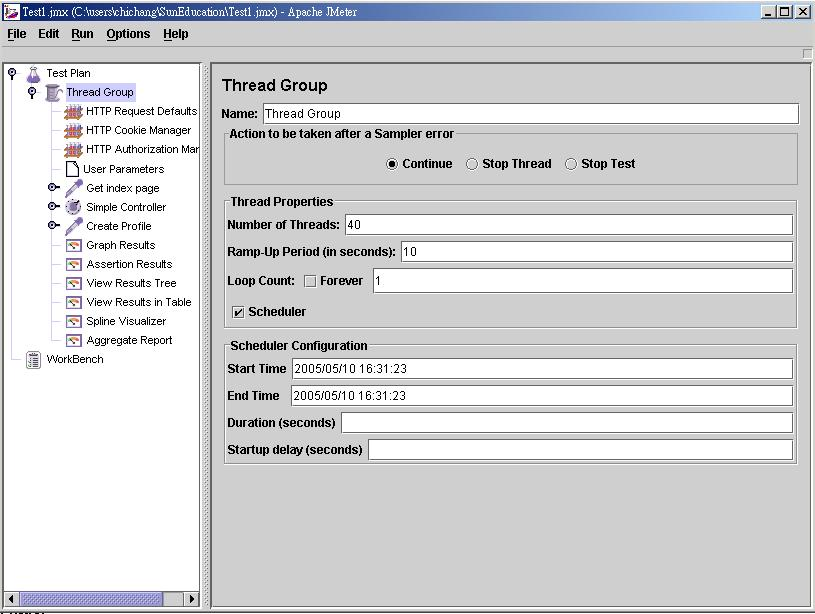
\includegraphics[width=400pt]{img/jmeter.jpg}
\end{center}
\caption{Interface de JMeter}
\label{jmeter_scenario}
\end{figure}

\subsubsection{LoadUI}
LoadUI\cite{www_loadui} est un projet de la société SmartBear (anciennement Eviware) qui a créé le logiciel SoapUI\cite{www_soapui} utilisé pour tester des webservices de manière fonctionnelle. LoadUI a été créé suite à une forte demande de la communauté d'utilisateurs de SoapUI et intègre donc logiquement ce dernier. Son interface utilise JavaFX et est très soignée, à l'inverse de JMeter comme le montre la Figure \ref{loadui_ui}.

\begin{figure}[ht]
\begin{center}
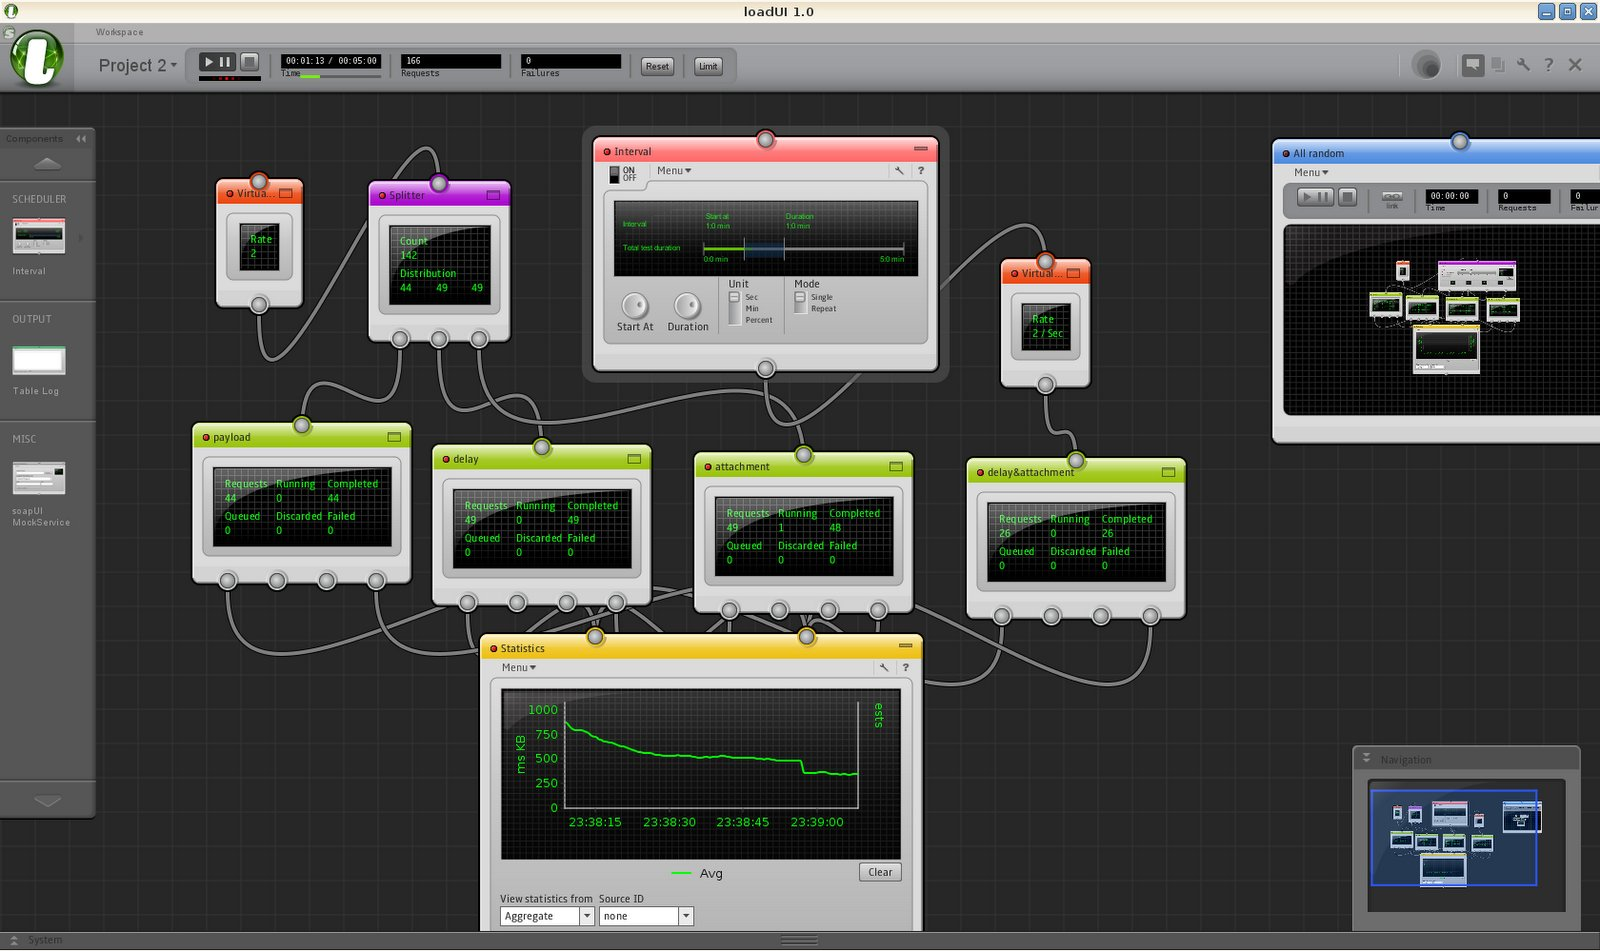
\includegraphics[width=400pt]{img/loadui.jpg}
\end{center}
\caption{Interface de LoadUI}
\label{loadui_ui}
\end{figure}

\subsection{Limitations des outils actuels}
Les outils disponibles pour faire du test de charge fonctionnent bien mais ont quelques lacunes.
\subsubsection{Interface Graphique}
Les outils tels que JMeter ou LoadUI ne proposent qu'une façon de créer des scénarios et de les exécuter : via une interface graphique. Il n'y a aucun moyen de passer outre et si l'on veut modifier les fichiers sources des scénario à la main $-$ si l'on n'a pas accès au logiciel, par exemple $-$, cela se révèle complexe car les fichiers n'ont pas été prévus pour être lisible par l'homme, mais pas des ordinateurs.

\subsubsection{Vocabulaire utilisé}
De plus, ces interfaces graphiques contiennent beaucoup de notions que l'utilisateur doit maîtriser en plus de l'application à tester. Par exemple, pour LoadUI, on trouve des \en{load generators}, des \en{runners}, etc. Les développeurs de JMeter, quant à eux, ont proposé un vocabulaire plus proche de l'implémentation de leur application que du domaine visé par l'application : \en{Thread Groups}, \en{Controllers}, \en{Listeners}, etc.

\subsubsection{Performances}
\label{pb_perfs}
Afin d'effectuer des tests de charge significatifs, il faut être capable de simuler un grand nombre d'utilisateurs ou de requêtes par seconde. Les outils existants consomment beaucoup de mémoire et de puissance CPU et proposent une solution afin de remédier à ce problème : la distribution des tests sur plusieurs machines. Cela induit donc des coûts supplémentaires. De plus, cela oblige le testeur à surveiller ces différentes machines afin de vérifier que le test lancé soit vraiment significatif. En effet, si un des agents de test plante ou ralentit pour une raison quelconque, le test effectué ne fournira pas les résultats attendus.

\subsection{Gatling}
Le projet Gatling naît donc d'une volonté d'aller au-delà de ces limitations et de proposer à ses futurs utilisateurs un logiciel :
\begin{itemize}
  \item \em{Performant}. Gatling permettra d'effectuer des tests complexes et lourds en utilisant le moins de ressources possible, grâce à l'optimisation de ses performances. Ceci étant la raison principale motivant sa création.
  \item \em{Simple d'utilisation}. Gatling offrira une interface utilisateur simple et rapide à prendre en main.
  \item \em{Accessible}. Gatling utilisera un vocabulaire proche du domaine du test de charge.
\end{itemize}